\section{Data split}

At the start of the project, the dataset was split into a training set and a
test set in a 90:10 proportion. Ideally, the train and test sets would have
the same distribution of classes, but the limited amount of data made this
more difficult. As can be seen from figure (\ref{lang-vs-cefr}), 15 of the
combinations \(L\times C\) have three or fewer occurences.

\begin{figure}
  \centering
  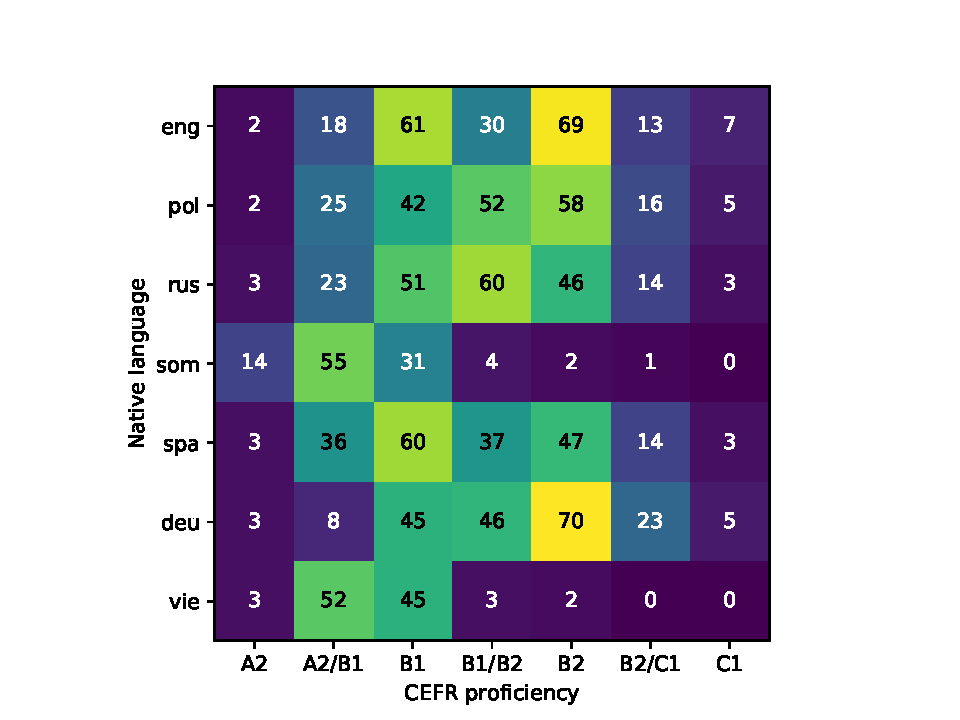
\includegraphics[width=0.8\textwidth]{lang_vs_cefr}
  \caption{The distribution of proficiency scores for each L1}
  \label{lang-vs-cefr}
\end{figure}
